\subsection{Rectas}

\begin{postulate}
    Existe al menos una recta, y se representa por:
    
    \begin{figure}[h]
        \centering
        \begin{tikzpicture}[scale=1] 
    \tkzInit[xmax=6,ymax=2, xstep=1]
    
    \tkzDefPoints{% x    y   nombre
                    0  /0   /A,
                    6  /0   /B}
    
    \tkzDrawLine[black,Latex-Latex](A,B)
    \tkzLabelLine[style={above}, pos=1](A,B){$l$}
\end{tikzpicture}
        \caption{Recta $l$}
        \label{fig:plot1}
    \end{figure}
\end{postulate}

\begin{postulate}
    Dada una recta $m$ existe al menos un punto $P$ que no pertenece a $m$.
    
    \begin{figure}[h]
        \centering
        \begin{tikzpicture}[scale=1] 
    \tkzInit[xmax=6,ymax=2, xstep=1]
    
    \tkzDefPoints{% x    y   nombre
                    0  /0   /A,
                    6  /0   /B,
                    2  /1   /P}
    
    \tkzDrawPoint(P)
    \tkzLabelPoint[right](P){$P$}
    \tkzDrawLine[black,Latex-Latex](A,B)
    \tkzLabelLine[style={above}, pos=1](A,B){$m$}
\end{tikzpicture}
        \caption{$P \notin m$}
        \label{fig:plot2}
    \end{figure}
\end{postulate}

\begin{postulate}
    Existe una y solo una recta que pasa por dos puntos distintos $A$ y $B$. Se escribe $\lne{AB}$ y se lee ``recta AB''. 
    
    \begin{figure}[h]
        \centering
        \begin{tikzpicture}[scale=1] 
    \tkzInit[xmax=6,ymax=2, xstep=1]
    
    \tkzDefPoints{% x    y   nombre
                    0  /0   /A,
                    6  /0   /B}
    
    \tkzDrawPoints(A,B)
    \tkzLabelPoints[below](A,B)
    \tkzDrawLine[black,Latex-Latex](A,B)
\end{tikzpicture}
        \caption{$\lne{AB}$}
        \label{fig:plot3}
    \end{figure}
\end{postulate}

\begin{postulate}
    En una recta existen al menos dos puntos $A$ y $B$.
    
    \begin{figure}[!h]
        \centering
        \begin{tikzpicture}[scale=0.8] 
    \tkzInit[xmax=5,ymax=0] 
    \tkzDrawX[label={}]
    \tkzDefPoints{0/0/FA,3/0/FP,0/1/A,3/1/P,5/1/B}
    
    \tkzDrawPoints(FA,FP,A,P)
    \tkzLabelPoint[above](A){$P$}
    \tkzLabelPoint[above](P){$Q$}
    \tkzDrawLine[black,Latex-Latex](A,B)
    \tkzLabelLine[above right,pos=1](A,B){$l$}
    \tkzLabelPoint[above](FA){$c(P)$}
    \tkzLabelPoint[above](FP){$c(Q)$}
    \tkzLabelPoint[below](FA){$0$}
    \tkzLabelPoint[below](FP){$x$}
\end{tikzpicture}
        \caption{$\lne{AB}$}
        \label{fig:plot4}
    \end{figure}
\end{postulate}

\begin{postulate}[\textbf{Postulado de rectas paralelas:}]
    Por un punto exterior a una recta dada se puede trazar una recta única que sea paralela a ella. Dos rectas son paralelas si están en un mismo plano y su intersección es vacía i.e. $l \cap m = \emptyset$.
    
    \begin{figure}[!h]
        \centering
        \begin{tikzpicture}[scale=1] 
\tkzInit[xmax=6,ymax=2, xstep=1]

\tkzDefPoints{% x    y   name
                0  /0   /A,
                6  /1   /B,
                0  /1   /C,
                6  /2   /D,
                3  /1.5 /P}

\tkzDrawLine[black,Latex-Latex](A,B)
\tkzDrawLine[black,Latex-Latex](C,D)
\tkzLabelLine[style={above right}, pos=1](A,B){$m$}
\tkzLabelLine[style={above right}, pos=1](C,D){$l$}

\tkzDrawPoint(P)
\tkzLabelPoints[above](P)

\end{tikzpicture}
        \caption{Rectas Paralelas}
        \label{fig:plot15}
    \end{figure}

    Dicho de otra manera, dada una recta $m$ y un punto $P$ exterior a ella, la recta $l$, paralela a ella, y que pasa por el punto exterior $P$, es única.
    
\end{postulate}

\clearpage

\begin{theorem}

Si dos rectas distintas se intersecan, su intersección contiene solamente un punto. Es decir, dos rectas no pueden tener más que un solo punto en común, i.e. $l \cap m = \{P\}$.

    \begin{figure}[!h]
        \centering
        \begin{tikzpicture}[scale=1] 
\tkzInit[xmax=6,ymax=2, xstep=1]

\tkzDefPoints{% x    y   name
                0  /0    /A,
                6  /1    /B,
                0  /2    /C,
                6  /0    /D,
                4  /0.67 /P}

\tkzDrawLine[black,Latex-Latex](A,B)
\tkzDrawLine[black,Latex-Latex](C,D)
\tkzLabelLine[style={above right}, pos=1](A,B){$m$}
\tkzLabelLine[style={above right}, pos=-0.1](C,D){$l$}

\tkzDrawPoint(P)
\tkzLabelPoints[above](P)

\end{tikzpicture}
        \caption{$l \cap m = \{P\}$}
        \label{fig:plot19}
    \end{figure}
    
\end{theorem}

\clearpage

\subsection{Planos}

\begin{definition}[\textbf{Puntos Coplanares}]
Cuatro o más puntos son \textit{coplanares} si pertenecen a un mismo plano.
\end{definition}

\begin{definition}[\textbf{Puntos No Coplanares}]
Cuatro o más puntos que no están en el mismo plano reciben el nombre de puntos \textit{no complanares}.
\end{definition}

\begin{postulate}
    Dados tres puntos no colineales, existe uno y solo un plano que los contiene.
    
    \begin{figure}[!h]
        \centering
        \begin{tikzpicture}[scale=1] 
    \tkzDefPoints{0/0/W,4/0/X,5/2/Y} 
    \tkzDefParallelogram(W,X,Y)
    
    \tkzGetPoint{Z}
    \tkzDrawPolygon(W,X,Y,Z)
    
    \tkzDefPoints{% x    y    nombre
                    1    /1    /A,
                    2.5  /1.5  /B,
                    3.5  /.5   /C,
                    4.2  /1.9  /P}
    
    \tkzDrawPoints(A,B,C)
    \tkzLabelPoint[below](A){$A$}
    \tkzLabelPoint[right](B){$B$}
    \tkzLabelPoint[right](C){$C$}
    
    \tkzLabelPoint[below right](P){$\pi$}
\end{tikzpicture}
        \caption{Puntos colineales}
        \label{fig:plot5}
    \end{figure}
\end{postulate}

\begin{postulate}
    Sobre un plano cualquiera existen al menos tres puntos no colineales.
    
    \begin{figure}[!h]
        \centering
        \begin{tikzpicture}[scale=1] 

\tkzDefPoints{0/0/W,4/0/X,5/2/Y} 
\tkzDefParallelogram(W,X,Y)

\tkzGetPoint{Z}
\tkzDrawPolygon(W,X,Y,Z)

\tkzDefPoints{% x    y    name
                1    /1    /A,
                2.5  /1.5  /B,
                3.5  /.5   /C,
                4.2  /1.9  /P}

\tkzDrawPoints(A,B,C)
\tkzLabelPoint[below](A){$E$}
\tkzLabelPoint[right](B){$D$}
\tkzLabelPoint[right](C){$F$}

\tkzLabelPoint[below right](P){$\sigma$}


\end{tikzpicture}
        \caption{Puntos no colineales}
        \label{fig:plot6}
    \end{figure}
\end{postulate}

\begin{postulate}
    Para todo plano existe un punto $E$ tal que $E$ no está en el plano.
    
    \begin{figure}[!h]
        \centering
        \begin{tikzpicture}[scale=1] 

\tkzDefPoints{0/0/W,4/0/X,5/2/Y} 
\tkzDefParallelogram(W,X,Y)

\tkzGetPoint{Z}
\tkzDrawPolygon(W,X,Y,Z)

\tkzDefPoints{% x    y    name                
                2  /3      /E,
                4.2  /1.9  /P}

\tkzDrawPoints(E)
\tkzLabelPoint[right](E){$E$}
\tkzLabelPoint[below right](P){$\pi$}


\end{tikzpicture}
        \caption{Punto $E$ fuera del plano}
        \label{fig:plot7}
    \end{figure}
\end{postulate}

\clearpage

\begin{postulate}[\textbf{Dos puntos, la recta y el plano:}]
    Si dos puntos de una recta están en un plano, todos los puntos de la recta están en el plano. Simbólicamente si $\pt{A} \in \pi, \pt{B} \in \pi \imply \lne{AB} \in \pi$. En otras palabras, si una recta tiene dos puntos comunes con un plano, toda la recta está contenida en el plano.
    
    \begin{figure}[!h]
        \centering
        \begin{tikzpicture}[scale=1] 

\tkzDefPoints{0/0/W,4/0/X,5/2/Y} 
\tkzDefParallelogram(W,X,Y)

\tkzGetPoint{Z}
\tkzDrawPolygon(W,X,Y,Z)

\tkzDefPoints{% x     y     name                
                1.2  /.7    /A,
                3.7  /1.1   /B,
                4.2  /1.9   /P}

\tkzDrawPoints(A,B)
\tkzDrawLine[black,Latex-Latex](A,B)
\tkzLabelPoints[below](A,B)
\tkzLabelPoint[below right](P){$\pi$}

\end{tikzpicture}
        \caption{si $\pt{A} \in \pi, \pt{B} \in \pi \imply \lne{AB} \in \pi$}
        \label{fig:plot8}
    \end{figure}
    
\end{postulate}

\begin{postulate}
    Si dos planos tiene un punto en común también tiene una recta en común.
    
    \begin{figure}[!h]
        \centering
        \begin{tikzpicture}[scale=1] 

\tkzDefPoints{
%   X   Y     NAME  
    0   /0    /A,
    1   /2    /B,
    2   /2    /C,
    6   /0    /D,
    7   /2    /E,
    2   /3    /F,
    5   /3    /G,
    5   /2    /H,
    2   /0    /I,
    2   /-1   /J,
    5   /0    /K,
    5   /-1   /L,
    0   /1    /M,
    7   /1    /N,
    2   /1    /O,
    3.5 /1    /P,
    5   /1    /Q,
    6   /1.8  /S} 

\tkzDrawPoint(P)
\tkzLabelPoint(P){$P$}
\tkzLabelPoint[below right](S){$\sigma$}

\tkzDrawSegment(A,B)
\tkzDrawSegment(B,C)
\tkzDrawSegment(A,D)
\tkzDrawSegment(D,E)
\tkzDrawSegment(C,F)
\tkzDrawSegment(F,G)
\tkzDrawSegment(G,H)
\tkzDrawSegment(H,E)
\tkzDrawSegment(I,J)
\tkzDrawSegment(K,L)
\tkzDrawSegment(J,L)

\tkzDrawSegment(C,O)
\tkzDrawSegment(H,Q)

\tkzDrawSegment[dashed,lightgray](C,H)
\tkzDrawSegment[dashed,lightgray](I,O)
\tkzDrawSegment[dashed,lightgray](K,Q)

\tkzDrawLine[black,Latex-Latex](M,N)
\tkzLabelLine[style={below}, pos=1](M,N){$l$}

\end{tikzpicture}
        \caption{Punto y recta en común}
        \label{fig:plot9}
    \end{figure}
    
\end{postulate}

\begin{postulate}
    Así como un punto sobre una recta la separa en dos semirectas, también una recta separa a un plano en dos semiplanos y un plano separa el espacio en dos semiespacios.
    
    \begin{figure}[!h]
        \centering
        \begin{tikzpicture}[scale=1] 

\tkzDefPoints{0/0/W,4/0/X,5/2/Y} 
\tkzDefParallelogram(W,X,Y)

\tkzGetPoint{Z}
\tkzDrawPolygon(W,X,Y,Z)

\tkzDefPoints{% x     y     name                
                2    /0     /A,
                3    /2     /B,
                4.2  /1.9   /P,
                1    /0.5   /H1,
                3    /0.5   /H2}


\tkzDrawLine[black,Latex-Latex](A,B)
\tkzLabelLine[style={above left}, pos=1](A,B){$l$}

\tkzLabelPoint[below right](P){$\pi$}
\tkzLabelPoint[below](H1){\scriptsize{$H1$}}
\tkzLabelPoint[below](H2){\scriptsize{$H2$}}

\end{tikzpicture}
        \caption{Separación en semiplanos}
        \label{fig:plot16}
    \end{figure}
\end{postulate}

\clearpage

\begin{postulate}
    Si se tiene un plano $\pi$, una recta $l$ en el plano y un segmento cuyos extremos están en los dos semiplanos que determina $l$ en $\pi$, entonces el segmento interseca a la recta.
    
    \begin{figure}[!h]
        \centering
        \begin{tikzpicture}[scale=1] 
    \tkzDefPoints{0/0/W,4/0/X,5/2/Y} 
    \tkzDefParallelogram(W,X,Y)
    
    \tkzGetPoint{Z}
    \tkzDrawPolygon(W,X,Y,Z)
    
    \tkzDefPoints{% x     y     nombre                
                    2    /0     /A,
                    3    /2     /B,
                    4.2  /1.9   /P,
                    1    /0.5   /H1,
                    3    /0.5   /H2,
                    1.5  /1.5   /R,
                    3.8  /0.8   /S}
    
    \tkzDrawPoints(R,S)
    \tkzLabelPoint[below](R){$A$}
    \tkzLabelPoint[below](S){$B$}
    \tkzDrawSegment(R,S)
    
    \tkzDrawLine[black,Latex-Latex](A,B)
    \tkzLabelLine[style={below right}, pos=1](A,B){$m$}
    
    \tkzLabelPoint[below right](P){$\pi$}
    \tkzLabelPoint[below](H1){\scriptsize{$H1$}}
    \tkzLabelPoint[below](H2){\scriptsize{$H2$}}
\end{tikzpicture}
        \caption{Segmento interseca a la recta}
        \label{fig:plot17}
    \end{figure}

    Dicho de otra manera, dada una recta $m$ y un plano $\pi$ que la contiene, los puntos de plano que no están en $m$ forman dos conjuntos tales que:

    \begin{itemize}
        \item Cada uno de los conjuntos del plano es un conjunto convexo.
        \item Si un punto $A$ está en uno de los conjuntos, y un punto $B$ está en el otro, entonces el segmento $\seg{AB}$ interseca a la recta $m$.
    \end{itemize}
    
\end{postulate}

\begin{theorem}
    Dada una recta $m$ y un punto $A$ tal que $A \not \in m$, existe un plano que contiene a $A$ y $m$ y ese plano es único.
 
    \begin{figure}[!h]
        \centering
        \begin{tikzpicture}[scale=1] 

\tkzDefPoints{0/0/W,4/0/X,5/2/Y} 
\tkzDefParallelogram(W,X,Y)

\tkzGetPoint{Z}
\tkzDrawPolygon(W,X,Y,Z)

\tkzDefPoints{% x     y       name                
                1.5  /1.3    /H,
                3.5  /1.3    /G,
                2.5  /0.5    /A,
                4.2  /1.9    /P}

\tkzDrawPoints(H,G,A)
\tkzLabelPoints[below](H,G)
\tkzLabelPoints[right](A)


\tkzDrawLine[black,Latex-Latex](H,G)
\tkzLabelLine[style={above left}, pos=1](H,G){$m$}
\tkzLabelPoint[below right](P){$\pi$}

\end{tikzpicture}
        \caption{Plano único que contiene a $A$ y $m$}
        \label{fig:theorem1}
    \end{figure}
        
\end{theorem}

\begin{definition}[\textbf{Rectas Coplanares}]
Dos o más rectas en un mismo plano se denominal coplanares.
\end{definition}

\begin{definition}[\textbf{Rectas Paralelas}]
Dos o más rectas que no se intersecan se denominan \textit{paralelas}.
\end{definition}

\begin{definition}[\textbf{Rectas Concurrents}]
Dos o mas rectas coplanares que se intersecan en un mismo punto se denominan \textit{concurrentes}.
\end{definition}

\clearpage

\subsection{Puntos Colineales}

\begin{definition}[\textbf{Puntos Colineales}]
Tres o más puntos son colineales si pertenecen a una misma recta.
\end{definition}

\begin{definition}[\textbf{Puntos No Colineales}]
Si tres o más puntos no pertenecen a la misma recta se denominan \textit{no colineales}.
\end{definition}

\begin{postulate}
    Dados tres puntos colineales $A,B$ y $C$, de manera que $AB + BC = AC$, entonces se afirma que $B$ está entre $A$ y $C$.  Si el punto $B$ está entre $A$ y $C$, entonces $A,B,C$ son puntos colineales y distintos entre sí. Para indicar que $B$ está entre $A$ y $C$ se denota $A\,-\,B\,-\,C$.
    
    \begin{figure}[!h]
        \centering
        \begin{tikzpicture}[scale=1] 
    \tkzInit[xmax=6,ymax=2, xstep=1]
    
    \tkzDefPoints{% x    y   nombre
                    0  /0   /A,
                    3  /0   /B,
                    6  /0   /C}
    
    \tkzDrawPoints(A,B,C)
    \tkzLabelPoints[below](A,B,C)
    \tkzDrawLine[black,Latex-Latex](A,C)
\end{tikzpicture}
        \caption{Puntos colineales}
        \label{fig:plot10}
    \end{figure}
\end{postulate}

\begin{postulate}
    Si $A$ y $B$ son puntos distintos, existe al menos un punto $C$ tal que $A\,-\,C\,-\,B$ y al menos un punto $D$ tal que $A\,-\,B\,-\,D$.
    
    \begin{figure}[!h]
        \centering
        \begin{tikzpicture}[scale=1] 
\tkzInit[xmax=6,ymax=2, xstep=1]

\tkzDefPoints{% x    y   name
                0  /0   /A,
                3  /0   /C,
                6  /0   /B,
                9  /0   /D}

\tkzDrawPoints(A,B,C,D)
\tkzLabelPoints[below](A,B,C,D)
\tkzDrawLine[black,Latex-Latex](A,D)

\end{tikzpicture}
        \label{fig:plot11}
        \caption{Entre dos puntos}
    \end{figure}
\end{postulate}

\begin{postulate}
    Dados tres puntos colineales distintos, uno y solo uno está entre los otros dos.
    
    \begin{figure}[!h]
        \centering
        \begin{tikzpicture}[scale=1] 
    \tkzInit[xmax=6,ymax=2, xstep=1]
    
    \tkzDefPoints{% x    y   nombre
                    0  /0   /A,
                    1  /0   /B,
                    2  /0   /C,
                    4  /0   /D,
                    5  /0   /E,
                    6  /0   /F,
                    8  /0   /G,
                    9  /0   /H,
                    10 /0   /I}
    
    \tkzDrawPoints(A,B,C,D,E,F,G,H,I)
    \tkzLabelPoints[below](A,B,C)
    
    \tkzLabelPoint[below](D){$A$}
    \tkzLabelPoint[below](E){$C$}
    \tkzLabelPoint[below](F){$B$}
    
    
    \tkzLabelPoint[below](G){$C$}
    \tkzLabelPoint[below](H){$A$}
    \tkzLabelPoint[below](I){$B$}
    
    
    \tkzDrawLine[black,Latex-Latex](A,C)
    \tkzDrawLine[black,Latex-Latex](D,F)
    \tkzDrawLine[black,Latex-Latex](G,I)
\end{tikzpicture}
        \caption{Entre dos puntos}
        \label{fig:plot12}
    \end{figure}
    
\end{postulate}

\clearpage

\subsection{Distancia entre Puntos}

\begin{postulate}[\textbf{Postulado de la distancia}]
A cada par de puntos de un plano les corresponde un único número real mayor o igual que o, conocido como la distancia.
\end{postulate}

\begin{postulate}[\textbf{Postulado de dos puntos:}]
Si se tiene dos puntos $A$ y $B$, $A = B$, si y solamente si $AB = 0$.
Si se tienen dos puntos $C$ y $D$, entonces $CD = DC$
\end{postulate}

\begin{postulate}
La distancia más corta entre dos puntos es el segmento que les une.
\end{postulate}

\begin{theorem}
    Si se tienen tres puntos $F,G$ y $H$, entonces $FG + GH \ge FH$. En caso de que $F,G$ y $H$ no sean colineales se cumple que $FG + GH > FH$.

    \begin{corolary}
    La distancia más corta entre dos puntos es una línea recta.
    \end{corolary}
    
\end{theorem}

\begin{definition}[\textbf{Estar entre:}]
    Dados tres puntos colineales, $\pt{A,B,C}$, de manera que $\dist{AB} + \dist{BC} = \dist{AC}$, entonce se afirma que $\pt{B}$ \textit{está entre} $\pt{A}$ y $\pt{C}$ y se escribe $\pt{A \,- \,B \,- \, C}$.
\end{definition}

\begin{definition}[\textbf{Segmento congruente:}]
    Dos segmentos con la misma medida reciben el nombre de \textit{segmento congruentes}. Si $\seg{AB}$ es congruente con $\seg{CD}$ se escribe $\seg{AB} \cong \seg{CD}$.
\end{definition}

\begin{theorem}[\textbf{Teorema de construcción del segmento}]
    Dado un segmento $\seg{AB}$ y un rayo $\ray{CD}$, hay exactamente un punto $\pt{E}$ de $\ray{CD}$, tal que $\seg{AB} \cong \seg{CE}$.   

\end{theorem}

\clearpage

\subsection{Coordenadas}

\begin{postulate}[\textbf{Postulado de la Regla}]
    La distancia entre dos puntos dados es el valor absoluto de la diferencia de los dos números reales asociados a ellos (i.e. sus coordenadas).

    Esto se basa en las siguientes afirmaciones:
    
    \begin{itemize}
        \item A cada punto de la recta le corresponde un número real único, denominado coordenada de ese punto.
        \item A cada número real le corresponde exactamente un punto de la recta.    
    \end{itemize}

    Supongamos que existe una recta $l$ que contiene al punto $P$, y la coordenada de $P$ en $l$ es $x$, escribimos $c(P) = x$ para denotar su sistema de coordenadas $c$.
    
\end{postulate}

\begin{theorem}
    Sean $A$ y $P$ dos puntos de la recta $\lne{AB}$. Entonces $l = \lne{AB}$ tiene un sistema coordenado $f$ en el cual la coordenada de $A$ es $0$ y la de $P$ es un número positivo.

    \begin{figure}[!h]
        \centering
        \begin{tikzpicture}[scale=0.8] 
    \tkzInit[xmax=6,ymax=0] 
    \tkzDrawX[label={}]
    \tkzDefPoints{
        0 /0 /CA,
        3 /0 /CB,
        6 /0 /CC,
        0 /0 /A,
        3 /0 /B,
        6 /0 /C}
    
    \tkzDrawPoints(A,B,C,CA,CB,CC)
    
    \tkzLabelPoint[above](A){$A$}
    \tkzLabelPoint[above](B){$B$}
    \tkzLabelPoint[above](C){$C$}
    
    %\tkzDrawSegment[add=0.0 and 0.3, -Latex](A,C)
    
    \tkzLabelPoint[below](CA){$0$}
    \tkzLabelPoint[below](CC){$r$}
\end{tikzpicture}
        \caption{Sistema de Coordenadas}
        \label{fig:plot18}
    \end{figure}

\end{theorem}

\clearpage

\subsection{Plano y Espacio}

\begin{definition}[\textbf{Espacio:}]
El conjunto de todos los puntos recibe el nombre de \textit{espacio}. Se acostumbra denotarlo con la letra $S$.
\end{definition}

\begin{postulate}
El espacio contiene, al menos, cuatro puntos diferentes no coplanares.
\end{postulate}

\begin{postulate}
    En el espacio, si se tiene un plano y un segmento con extremos en los dos semiplanos, el segmento interseca al plano.
\end{postulate}

\begin{definition}[\textbf{Conjunto convexo:}]
    Un conjunto $A$ se llama \textit{convexo} si para cada par de puntos $\pt{R}$ y $\pt{S}$, que pertenece a él, el segmento $\seg{RS}$ está contenido en $A$.

    \begin{figure}[h!]

        \centering

        \begin{subfigure}[b]{.5\textwidth}
            \centering
            \begin{tikzpicture}[scale=0.8] 


\tkzDefPoints{% x     y    name
                0    /0    /A,
                6    /0    /B,
                5    /6    /C,
                1    /5    /D,
                1.5  /1.5  /R,
                4    /4.5  /S}

\tkzDrawPolygon(A,B,C,D)
\tkzDrawPoints(R,S)
\tkzLabelPoints(R,S)
\tkzDrawSegment(R,S)

\end{tikzpicture}
            \label{fig:conjunto-convexo}
            \caption{Convexo}            
        \end{subfigure}%
        \begin{subfigure}[b]{.5\textwidth}
            \centering
            \begin{tikzpicture}[scale=0.8] 


\tkzDefPoints{% x     y    name
                0    /3    /A,
                6    /0    /B,
                3    /3    /C,
                5    /5    /D,
                3.2  /3.7  /R,
                3.8  /1.8    /S}

\tkzDrawPolygon(A,B,C,D)
\tkzDrawPoints(R,S)
\tkzLabelPoints[left](R,S)
\tkzDrawSegment(R,S)

\end{tikzpicture}
            \label{fig:conjunto-no-convexo}
            \caption{No Convexo}            
        \end{subfigure}
        
        \centering
        \caption{Convexidad}
        \label{fig:convexidad}
    
    \end{figure}
    
\end{definition}

\begin{postulate}[\textbf{Postulado de separación del plano}]
    Dada una recta $m$ y un plano que la contiene, los puntos del plano que no están en $m$ forman dos conjuntos:

    \begin{itemize}
        \item Cada uno de los conjuntos del plano es un conjunto convexo.
        \item Si un punto $\pt{R}$ está en uno de los conjunots y punto $\pt{S}$ está en el otro, entonces el segmentos $\seg{RS}$ interseca a la recta $m$.
    \end{itemize}
\end{postulate}

\clearpage

\begin{definition}[\textbf{Arista:}]
    Una recta en el plano que determina dos conjuntos convexos llamados semiplanos se denomina \textit{arista} o \textit{borde} de cada uno de ellos.

    \begin{figure}[!h]
        \centering
        \begin{tikzpicture}[scale=1] 

\tkzDefPoints{0/0/W,5/0/X,6/4/Y} 
\tkzDefParallelogram(W,X,Y)

\tkzGetPoint{Z}
\tkzDrawPolygon(W,X,Y,Z)

%\tkzLabelPoints(W,X,Y,Z)

\tkzDefPoints{% x     y     name                
                1    /0.7    /A,
                4.5  /3.1    /B,
                5.2  /3.9    /P}

\tkzDrawPoints(A,B)
\tkzDrawLine[black,Latex-Latex](A,B)
\tkzLabelPoint[below right](P){$\pi$}
\tkzLabelSegment[above,style={sloped}](A,B){\footnotesize{Semiplano}}
\tkzLabelSegment[below,style={sloped}](B,A){\footnotesize{Semiplano}}

\end{tikzpicture}
        \caption{Arista}
        \label{fig:arista}
    \end{figure}
    
\end{definition}

\begin{postulate}[\textbf{Separación del espacio}]
    Los puntos del espacio que no están en un plano dado forman dos conjuntos denominados semiespacios tales que:

    \begin{itemize}
        \item Los dos conjuntos, uno a cada lado del plano, son convexos.
        \item Si un punto $\pt{R}$ está en uno de los conjuntos y punto $\pt{S}$ está en el otro, entonces el segmentos $\seg{RS}$ interseca al plano en un punto.
    \end{itemize}
\end{postulate}
